\documentclass{beamer}

%%%%%%%%%%%%%Solarized Theme%%%%%%%%%%%%%%%
\usecolortheme[dark,accent=cyan]{solarized}
\beamertemplatenavigationsymbolsempty

%%%%%Packages%%%%%
\usepackage{graphicx}
\graphicspath{ {static/} }

\usepackage{hyperref}
\usepackage{colortbl, xcolor}
\usepackage{booktabs}

\usepackage{tikz}
\usepackage{standalone}
\usetikzlibrary{decorations.pathmorphing, decorations.markings, arrows}
\usetikzlibrary{decorations.pathreplacing,angles,quotes, calc, er, positioning}

\usepackage{amsmath}
\usepackage{amsthm}
\usepackage{amssymb}
\usepackage[framemethod=TikZ]{mdframed}
\setbeamertemplate{blocks}[default]

\mdfdefinestyle{framed}{%
    linecolor=orange,
    outerlinewidth=2pt,
    roundcorner=10pt,
    innertopmargin=10pt,
    innerbottommargin=10pt,
    innerrightmargin=8pt,
    innerleftmargin=8pt,
    backgroundcolor=solarizedBase03}

\mdfdefinestyle{blank}{%
    linecolor=solarizedBase03,
    outerlinewidth=2pt,
    roundcorner=10pt,
    innertopmargin=10pt,
    innerbottommargin=10pt,
    innerrightmargin=8pt,
    innerleftmargin=8pt,
    backgroundcolor=solarizedBase03}

\usetikzlibrary{shapes.arrows, positioning, arrows, decorations.pathreplacing,
angles, quotes, decorations.pathmorphing}
%%%%%%Title%%%%%%%%
\title{Memory Size in the Prisoner's Dilemma}
\author{Nikoleta E. Glynatsi}
\date{\small{Dr. Vincent \textsc{Knight} \hspace{1cm} 
Dr. Jonathan \textsc{Gillard} }}
\institute[]
{
\begin{center}
    
\includegraphics[width=.20\textwidth]{cardiff_uni_logo.jpg}
\end{center}
}

\begin{document}

\maketitle

\begin{frame}
    \centering
    
\includegraphics[width=.2\textwidth]{players} \hspace{.6cm}
    
\includegraphics[width=.2\textwidth]{actions} \hspace{.6cm}
    
\includegraphics[width=.2\textwidth]{objective}
\end{frame}

\begin{frame}
    \centering
    \includestandalone[width=.8\textwidth]{matrix}
\end{frame}

\begin{frame}
    \centering
    \includestandalone[width=.7\textwidth]{memory_one}
\end{frame}

\begin{frame}
    \begin{center}
    \textcolor{orange}{\textbf{
    \underline{William H. Press and Freeman J. Dyson.}
    Iterated Prisoner's Dilemma contains strategies that dominate any evolutionary
    opponent. \underline{2012}}}
    \end{center}
\end{frame}

\begin{frame}
    \centering
    \includestandalone[width=.7\textwidth]{achieve}
\end{frame}

\begin{frame}
    \begin{mdframed}[style=blank]
    \centering
    \large{
    \textbf{\textcolor{orange}{WHICH IS THE BEST MEMORY ONE STRATEGY?}}}
    \end{mdframed}
    \begin{mdframed}[style=blank]
    \centering
    \large{
    \textbf{\textcolor{orange}{ARE THERE LIMITATIONS TO MEMORY ONE STRATEGIES?}}}
    \end{mdframed}
\end{frame}

\begin{frame}
    \begin{mdframed}[style=framed]
    \centering
    \large{
    \textbf{\textcolor{orange}{WHICH IS THE BEST MEMORY ONE STRATEGY?}}}
    \end{mdframed}
    \begin{mdframed}[style=blank]
    \centering
    \large{
    \textbf{\textcolor{orange}{ARE THERE LIMITATIONS TO MEMORY ONE STRATEGIES?}}}
    \end{mdframed}
\end{frame}


\begin{frame}
    \centering
    \includestandalone[width=0.5\textwidth]{memory_one_chain}
  
    \vfill
    \textcolor{orange}{
    \large
    \boldmath\( p = (p_1, p_2, p_3, p_4) \in\mathbb{R}_{[0,1]}^{4} \)}
\end{frame}

\begin{frame}
    \centering
    \includestandalone[width=.7\textwidth]{states}
\end{frame}

\begin{frame}
    \centering
    \Large\textcolor{orange}{
    \boldmath \( \max_p u_q(p)\text{ such that }p\in\mathbb{R}_{[0,1]}^{4}\)}
\end{frame}

\begin{frame}
    \begin{center}
    \begin{theorem}
     \boldmath\[ u_q(p) = \frac{\frac{1}{2} p Q  p^T + c^T  p + a} 
    {\frac{1}{2} p \bar{Q} p^T + \bar{c}^T p + \bar{a}}\]

    \begin{itemize}
      \item \boldmath\(Q, \bar{Q} \in\mathbb{R}^{4 \times 4}\)
      \item \boldmath\(c, \bar{c}\in\mathbb{R}^{4 \times 1}\) 
      \item \boldmath\(a, \bar{a}\in\mathbb{R}\)  
   \end{itemize}
    \end{theorem}
    \end{center}
\end{frame}

\begin{frame}
    \begin{center}
    \begin{theorem}
    {\tiny
     \boldmath\[\frac{1}{N} \sum\limits_{i=1} ^ {N} {u_q}^{(i)} (p) = \frac{1}{N}
     \frac{\sum\limits_{i=1} ^ {N} (\frac{1}{2} pQ^{(i)} p^T + c^{(i)T} p + a^ {(i)})
     \prod\limits_{\tiny\begin{array}{l} j=1 \\ j \neq i \end{array}} ^ 
     N (\frac{1}{2} p\bar{Q}^{(i)} p^T + \bar{c}^{(i)T} p + \bar{a}^ {(i)})}
     {\prod\limits_{i=1} ^ N (\frac{1}{2} p\bar{Q}^{(i)} p^T + \bar{c}^{(i)T} p + \bar{a}^ {(i)})}\]}
    \end{theorem}
    \end{center}
\end{frame}

\begin{frame}
    \centering
    
\includegraphics[width=.22\textwidth]{apple} \pause \hspace{2cm} 
    
\includegraphics[width=.3\textwidth]{tree} 
\end{frame}

\begin{frame}
    \begin{center}
    \includestandalone[width=.4\textwidth]{cube}
    \end{center}
\end{frame}

\begin{frame}
    \begin{center}
    \includestandalone[width=.4\textwidth]{cube_two}
    \end{center}
\end{frame}

\begin{frame}
    \begin{center}
    \includestandalone[width=.4\textwidth]{cube_three}
    \end{center}
\end{frame}

\begin{frame}
    \begin{center}
    \Large{
    \textbf{\textcolor{orange}{PURELY RANDOM}} \vspace{1cm}

    \textcolor{orange}{\boldmath\( p = (p, p, p, p)\)}}
    \end{center}
\end{frame}

\begin{frame}
    \begin{columns}
        \begin{column}{.65\textwidth}
    \Large{\textcolor{orange}{
    \[\mathbf{S_q = U_{\substack{i=1}} ^ {2N} \lambda_i \cup \{0, 1\}}\] \vspace{1mm}
    \[\mathbf{1 \leq|S_{q(i)}| \leq 2N + 2}\]}}
        \end{column}

        \begin{column}{.5\textwidth}
            \vspace{1cm}

            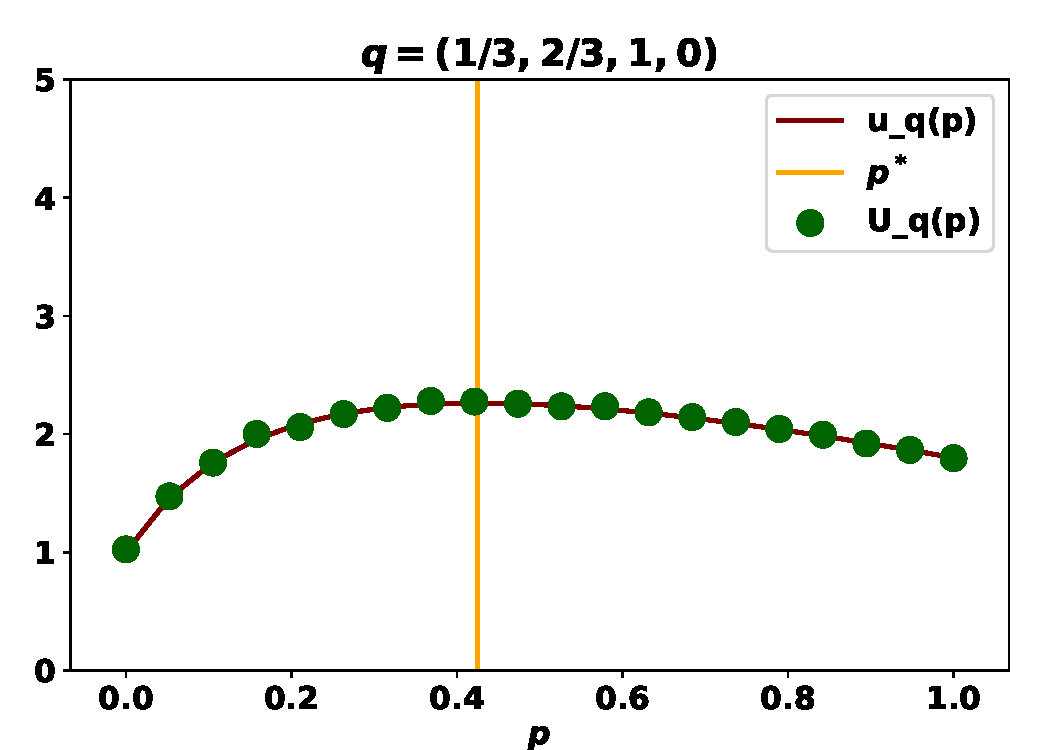
\includegraphics[width=.7\textwidth]{purely_random_match_two}

            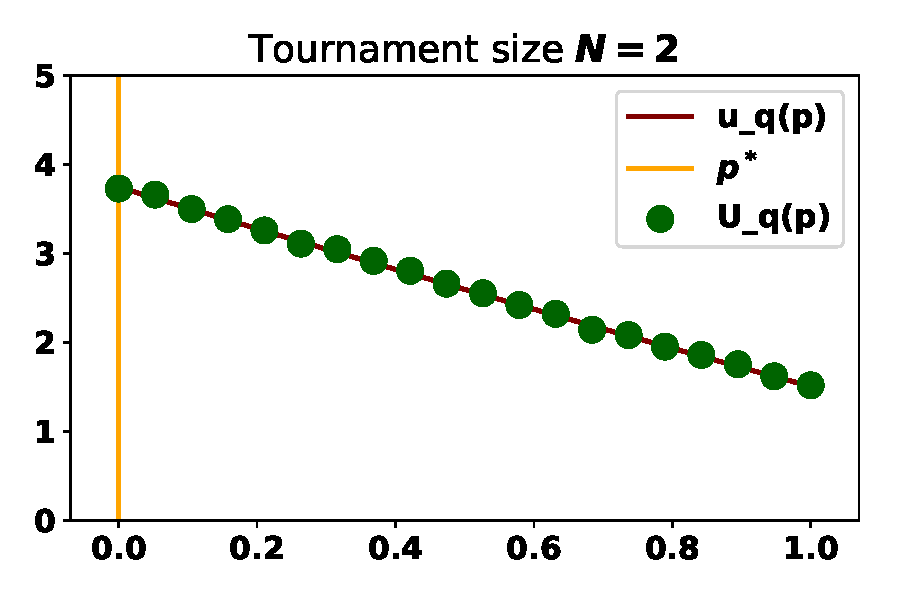
\includegraphics[width=.7\textwidth]{purely_random_tournament_one}
        \end{column}
    \end{columns}
    \pause
    \centering
    \vspace{1cm}
    \textbf{\textcolor{orange}{Result: optimal behaviour using eigenvalues of companion matrix}}
\end{frame}

\begin{frame}
    \begin{center}
    \Large{
    \textbf{\textcolor{orange}{REACTIVE}} \vspace{1cm}

    \textcolor{orange}{\boldmath\( p = (p_1, p_2, p_1, p_2)\)}}
    \end{center}
\end{frame}

\begin{frame}
    \begin{columns}
        \begin{column}{.5\textwidth}
            \includestandalone[width=\textwidth]{resultant}
        \end{column}
        \begin{column}{.5\textwidth}
            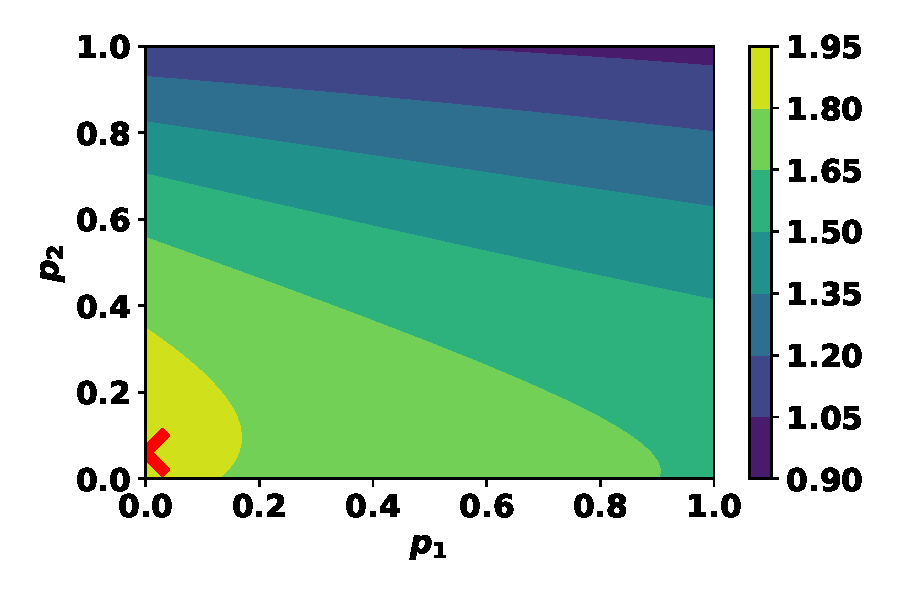
\includegraphics[width=\textwidth]{reactive_pairwise_one}
        \end{column}
    \end{columns}
    \pause
    \centering
    \vspace{2mm}
    \textbf{\textcolor{orange}{Result: optimal behaviour using Sylvester's resultant (Sylvester 1840)}}
\end{frame}

\begin{frame}
    \begin{center}
    \Large{
    \textbf{\textcolor{orange}{MEMORY ONE}}}
    \end{center}
\end{frame}

\begin{frame}
    \centering
    
\includegraphics[width=.2\textwidth]{work} \hspace{.6cm}
    
\includegraphics[width=.2\textwidth]{hill} \hspace{.6cm}
    
\includegraphics[width=.2\textwidth]{look}
\end{frame}

\begin{frame}
    \centering
    \textcolor{orange}{
    \resizebox{11cm}{!}{
    \begin{tabular}{lrrrrrrrrrrrrrrrlrr}
        \toprule
        {} &     $q_1$ &     $q_2$ &     $q_3$ &     $q_4$  &     $p_1$ &     $p_2$ &  $p_3$ &  $p_4$ &     $u_q$ &  $U_q$ \\
        \midrule
        0 &  0.208 & 0.481 & 0.420 & 0.859 & 0.603 & 0.435 & 0.0 & 0.0 & 3.494 & 3.467 \\
        1 &  0.781 & 0.692 & 0.969 & 0.032 & 0.000 & 0.000 & 0.0 & 1.0 & 3.266 & 3.328 \\
        2 &  0.546 & 0.964 & 0.063 & 0.383 & 0.389 & 0.491 & 0.0 & 0.0 & 4.659 & 4.544 \\
        3 &  0.930 & 0.381 & 0.665 & 0.999 & 0.145 & 0.480 & 0.0 & 0.0 & 3.470 & 3.454 \\
        4 &  0.309 & 0.129 & 0.346 & 0.770 & 0.566 & 0.039 & 0.0 & 0.0 & 2.878 & 2.886 \\
        \bottomrule
        \end{tabular}}}
\end{frame}


\begin{frame}
    \begin{mdframed}[style=blank]
    \centering
    \large{
    \textbf{\textcolor{orange}{WHICH IS THE BEST MEMORY ONE STRATEGY?}}}
    \end{mdframed}
    \begin{mdframed}[style=framed]
    \centering
    \large{
    \textbf{\textcolor{orange}{ARE THEIR LIMITATIONS TO MEMORY ONE STRATEGIES?}}}
    \end{mdframed}
\end{frame}

\begin{frame}
    \begin{center}
    \includestandalone[width=\textwidth]{limitations}
    \end{center}
\end{frame}

\begin{frame}
    \centering
    \textcolor{orange}{
    \resizebox{11cm}{!}{
    \begin{tabular}{lrrrrrrrrrrrrrrr}
    \toprule
    {} &     $q_1$ &     $q_2$ &     $q_3$ &     $q_4$ &  $\bar{q}_1$ &  $\bar{q}_2$ &  $\bar{q}_3$ &  $\bar{q}_4$ &  $p_1$ &  $p_2$ &  $p_3$ &     $p_4$ &     $u_q$ &   $U_q$ &  $U_{G}$ \\
    \midrule
    1 &  0.548 &  0.715 &  0.602 &  0.544 &      0.545 &     0.171 &     0.852 &     0.180 &    0.0 &    0.0 &    0.0 &  0.317 &  2.694 &  2.662 &   2.723 \\
    3 &  0.548 &  0.715 &  0.602 &  0.544 &      0.545 &     0.171 &     0.852 &     0.180 &    0.0 &    0.0 &    0.0 &  0.427 &  2.692 &  2.662 &   2.796 \\
    5 &  0.548 &  0.715 &  0.602 &  0.544 &      0.545 &     0.171 &     0.852 &     0.180 &    0.0 &    0.0 &    0.0 &  0.427 &  2.692 &  2.662 &   2.915 \\
    7 &  0.548 &  0.715 &  0.602 &  0.544 &      0.545 &     0.171 &     0.852 &     0.180 &    0.0 &    0.0 &    0.0 &  0.427 &  2.692 &  2.662 &   2.915 \\
    9 &  0.548 &  0.715 &  0.602 &  0.544 &      0.545 &     0.171 &     0.852 &     0.180 &    0.0 &    0.0 &    0.0 &  0.427 &  2.692 &  2.662 &   2.915 \\
            \bottomrule
            \end{tabular}}}
\end{frame}

\begin{frame}
    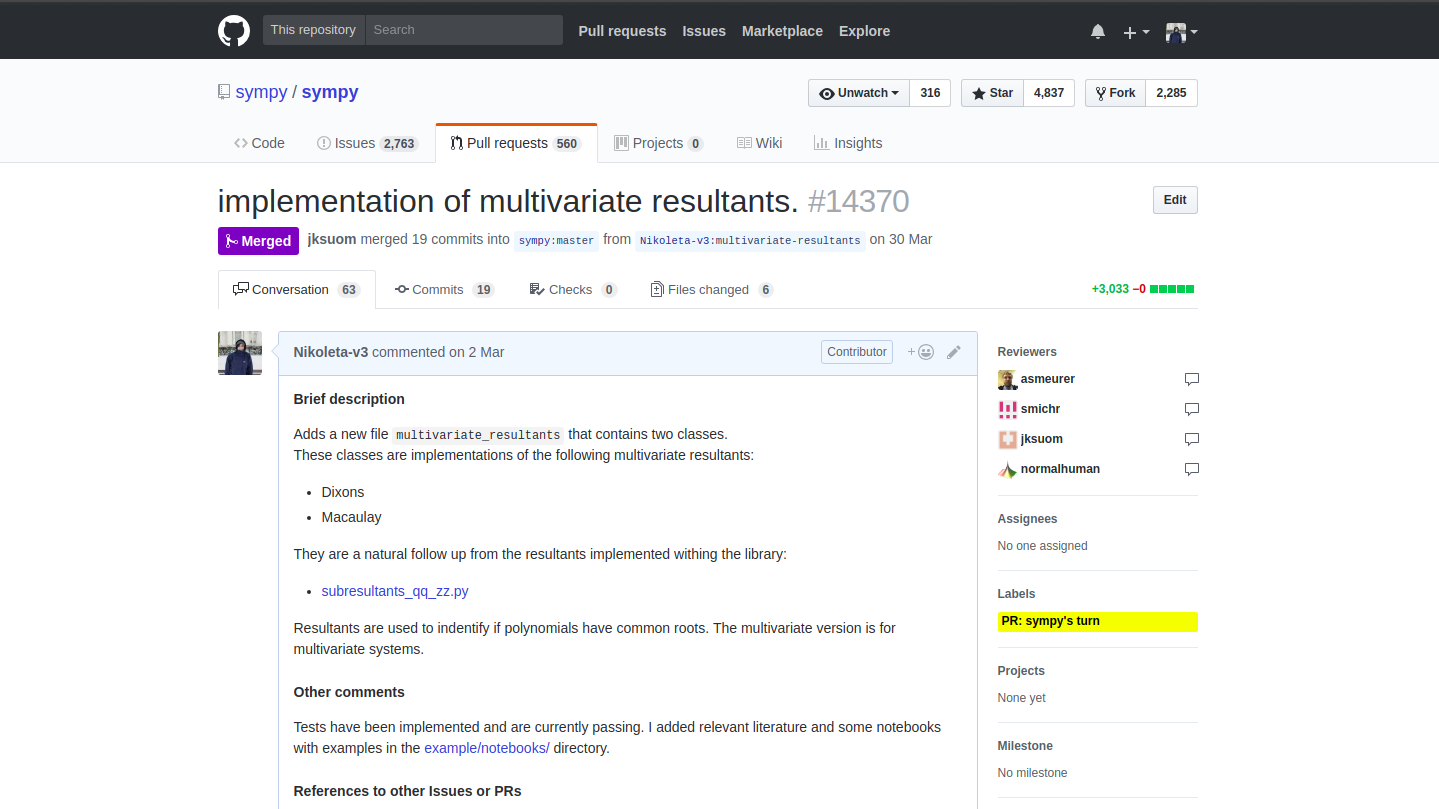
\includegraphics[width=\textwidth]{contribution}
\end{frame}

\begin{frame}
    \centering
    \large{\textcolor{orange}{\textbf{Limitations of memory size on the Iterated Prisoner's dilemma}. (In preparation)}} \\
    \vspace{2cm}

    \large \textbf{\textcolor{orange}{{@NikoletaGlyn}}}\\
    \large \textbf{\textcolor{orange}{{https://github.com/Nikoleta-v3}}}\\
\end{frame}

\end{document}
